% !TEX program = xelatex
\documentclass[UTF8,11pt,a4paper]{ctexart}
\usepackage[margin=2.1cm]{geometry}
\usepackage{graphicx,longtable,booktabs,array,hyperref,xcolor,fancyhdr,pdfpages}
\usepackage{calc,amssymb}
\setlength{\headheight}{15pt}
\hypersetup{colorlinks=true,linkcolor=teal,urlcolor=teal}
\setlength{\emergencystretch}{3em}
\setlength{\parskip}{0.35em}
\providecommand{\tightlist}{\setlength{\itemsep}{0pt}\setlength{\parskip}{0pt}}
\providecommand{\pandocbounded}[1]{#1}
\pagestyle{fancy}\fancyhf{}\fancyhead[L]{Wylie College · 软件工程课程设计}\fancyhead[R]{学习参考版 1.0}
\fancyfoot[L]{ClawsGO Science Agent}\fancyfoot[R]{\thepage}
\begin{document}


\includepdf[pages=1]{封面-单页排版适配.pdf}
\begin{titlepage}\vspace*{2cm}
{\Huge\bfseries 课程注册系统}\par\vspace{0.5cm}
{\LARGE 软件工程项目文档汇编}\par\vspace{1cm}
{\large 五人协作 · 需求追踪 · 事务一致性 · 可复现测试}\par\vspace{1cm}
版本：1.0 学习参考版\\日期：2026年10月10日\\编制：ClawsGO Science Agent
\vfill
\textbf{填写说明}：实际成员信息、贡献比例、签名与工作总结由团队据实填写。
\end{titlepage}\tableofcontents\clearpage
\clearpage
\hypertarget{ux9605ux8bfbux4e0eux6838ux9a8cux6307ux5357}{%
\section{阅读与核验指南}\label{ux9605ux8bfbux4e0eux6838ux9a8cux6307ux5357}}

Wylie College 课程注册系统｜五人课程设计学习参考包｜2026-10-10

\hypertarget{ux6750ux6599ux4f9dux636e}{%
\subsection{材料依据}\label{ux6750ux6599ux4f9dux636e}}

\begin{enumerate}
\def\labelenumi{\arabic{enumi}.}
\tightlist
\item
  《2026年软件工程课程设计要求.ppt》：五人一组；开发计划、需求、设计、测试计划、测试报告、个人与团队总结；可选配置管理；贡献百分比和签名；最后检查运行。
\item
  《2026年软件工程课程设计题目.pdf》：Wylie College Course Registration
  System，问题陈述、术语、补充规约和8个用例，共19页。
\item
  《2026-SECD-文档提交封面模板.docx》：保留原版封面供实际填写。模板有6行，五人组使用前5行，第6行留空或标注不适用。
\end{enumerate}

\hypertarget{ux4ea4ux4ed8ux72b6ux6001}{%
\subsection{交付状态}\label{ux4ea4ux4ed8ux72b6ux6001}}

代码为可运行学习参考实现，自动化测试结果单独留档。文档阐明已经实现的行为、建议计划和待确认差异。标注``建议''\,``待填''的内容不是已经发生的团队工作。

五位成员应核对领域模型、注册状态机与事务边界，保存设计决策、修改、测试和评审记录。

\hypertarget{ux63a8ux8350ux9605ux8bfbux8defux5f84}{%
\subsection{推荐阅读路径}\label{ux63a8ux8350ux9605ux8bfbux8defux5f84}}

\begin{itemize}
\tightlist
\item
  运行：代码目录 README → 初始化 → 三角色登录。
\item
  理解软件工程：01开发计划 → 02需求分析 → 03设计 → 04测试计划 →
  05测试报告。
\item
  团队组织：07分工咬合与接口契约 → 08答辩指南 → 09总结待填模板。
\item
  提交前：10验收清单 → 教师确认差异 → 填写封面。
\end{itemize}

\hypertarget{ux63d0ux4ea4ux524dux5fc5ux987bux89e3ux51b3ux7684ux53e3ux5f84}{%
\subsection{提交前必须解决的口径}\label{ux63d0ux4ea4ux524dux5fc5ux987bux89e3ux51b3ux7684ux53e3ux5f84}}

\begin{enumerate}
\def\labelenumi{\arabic{enumi}.}
\tightlist
\item
  首次提交是否严格要求4首选2备选；当前允许1--4首选、0--2备选。
\item
  ``关闭注册''和``学期教学结束''是否分开；当前以最近已关闭学期作为成绩录入学期。
\item
  备选允许与首选冲突，但补位时重新检查；原文没有明确定义备选同时检查的范围。
\item
  计费采用注册关闭后最终课表；问题陈述中的``学生完成注册后计费''与详细关闭用例存在表述差异，本实现优先详细用例。
\item
  Web替代旧桌面界面依据课程要求第2页；SQLite及模拟遗留系统不等于真实Ingres与账务对接。
\item
  原始2000/500用户指标、7×24可用性需另行验证，本包不宣称达标。
\end{enumerate}

ClawsGO Science Agent

\clearpage
\hypertarget{ux5f00ux53d1ux8ba1ux5212}{%
\section{开发计划}\label{ux5f00ux53d1ux8ba1ux5212}}

项目：Wylie College课程注册系统｜版本1.0｜计划参考稿

\hypertarget{1-ux76eeux6807ux4e0eux8303ux56f4}{%
\subsection{1. 目标与范围}\label{1-ux76eeux6807ux4e0eux8303ux56f4}}

以8个原始用例为范围边界，完成``人员建档---授课认领---学生注册---注册关闭---计费---成绩''闭环。选择分层单体，避免微服务、复杂权限平台、消息中间件等超出教学目标的设计。重点呈现需求澄清、模型驱动设计、接口约定、事务一致性、测试分层和配置管理。

交付质量门：安装可复现；用例主流可演示；关键异常有回归测试；文档与代码一致；未实现或未验证指标明确；每名成员能够解释自己和上下游接口。

\hypertarget{2-ux5efaux8baeux4e94ux4ebaux5de5ux4f5cux91cf}{%
\subsection{2.
建议五人工作量}\label{2-ux5efaux8baeux4e94ux4ebaux5de5ux4f5cux91cf}}

建议总投入200人时、每人40人时。该数值是后续自主实现/核验的估算，实际工时与贡献不得直接套用。

\textbf{A 架构与集成}

\begin{itemize}
\tightlist
\item
  分析/设计：10h
\item
  实现/自主改造：12h
\item
  测试/联调：10h
\item
  文档/答辩：8h
\item
  合计：40h
\end{itemize}

\textbf{B 人员生命周期}

\begin{itemize}
\tightlist
\item
  分析/设计：8h
\item
  实现/自主改造：14h
\item
  测试/联调：10h
\item
  文档/答辩：8h
\item
  合计：40h
\end{itemize}

\textbf{C 注册核心}

\begin{itemize}
\tightlist
\item
  分析/设计：10h
\item
  实现/自主改造：16h
\item
  测试/联调：8h
\item
  文档/答辩：6h
\item
  合计：40h
\end{itemize}

\textbf{D 授课与成绩}

\begin{itemize}
\tightlist
\item
  分析/设计：10h
\item
  实现/自主改造：14h
\item
  测试/联调：10h
\item
  文档/答辩：6h
\item
  合计：40h
\end{itemize}

\textbf{E 注册关闭与计费}

\begin{itemize}
\tightlist
\item
  分析/设计：10h
\item
  实现/自主改造：14h
\item
  测试/联调：10h
\item
  文档/答辩：6h
\item
  合计：40h
\end{itemize}

A承担跨模块集成与需求追踪的工作，B承担数据一致性与全组人员维护回归，C承担并发与回滚难点，D承担成绩到先修课的数据闭环，E承担关闭状态机及外部依赖故障。分工不以代码行数计算贡献。

\hypertarget{3-ux5efaux8baeux8fedux4ee3ux8bfeux7a0bux65f6ux6bb52026-09-08ux81f310-16}{%
\subsection{3.
建议迭代（课程时段2026-09-08至10-16）}\label{3-ux5efaux8baeux8fedux4ee3ux8bfeux7a0bux65f6ux6bb52026-09-08ux81f310-16}}

当前参考包在2026-10-10形成，下面早期日期用于说明完整项目应如何安排；不得补造这些日期的会议或提交记录。

\textbf{I0 范围与风险}

\begin{itemize}
\tightlist
\item
  建议时段：09-08---09-12
\item
  产出：用例目录、术语、差异记录、风险表
\item
  进入下一阶段的条件：教师确认关键口径；全员讲清边界
\end{itemize}

\textbf{I1 可走通骨架}

\begin{itemize}
\tightlist
\item
  建议时段：09-13---09-20
\item
  产出：工厂、数据库、登录、人员维护、缓存适配
\item
  进入下一阶段的条件：A→B账号集成测试通过
\end{itemize}

\textbf{I2 业务主链}

\begin{itemize}
\tightlist
\item
  建议时段：09-21---09-30
\item
  产出：选课、授课、成绩、关闭流程
\item
  进入下一阶段的条件：C→D花名册与D→C先修课对接通过
\end{itemize}

\textbf{I3 鲁棒性}

\begin{itemize}
\tightlist
\item
  建议时段：10-01---10-09
\item
  产出：并发测试、异常回滚、发件箱、故障注入
\item
  进入下一阶段的条件：最后一名额、目录故障、计费恢复通过
\end{itemize}

\textbf{I4 核验与答辩}

\begin{itemize}
\tightlist
\item
  建议时段：10-10---10-16
\item
  产出：自主修改、回归证据、真实总结、演练
\item
  进入下一阶段的条件：全部验收清单签字，材料一致
\end{itemize}

若从10月10日才开始：10日完成独立设计与差异确认；11--12日分模块自主实现/重构；13日联调；14日异常与回归；15日材料审核及两次演练；16日运行检查。压缩进度时优先保住用例主链与关键异常，扩展功能全部移出范围。

\hypertarget{4-ux98ceux9669ux4e0eux5e94ux5bf9}{%
\subsection{4. 风险与应对}\label{4-ux98ceux9669ux4e0eux5e94ux5bf9}}

\textbf{4+2含义不清}

\begin{itemize}
\tightlist
\item
  影响：验收不一致
\item
  预防 / 触发后的处理：记录CR-01；教师确认后集中改校验与用例
\item
  负责人：A+C
\end{itemize}

\textbf{并发超卖}

\begin{itemize}
\tightlist
\item
  影响：核心业务错误
\item
  预防 / 触发后的处理：写事务原子检查；最后名额竞态测试
\item
  负责人：C+A
\end{itemize}

\textbf{目录慢或离线}

\begin{itemize}
\tightlist
\item
  影响：大量页面不可用
\item
  预防 / 触发后的处理：快照缓存；明确失败页；隔离慢访问与写事务
\item
  负责人：A+D
\end{itemize}

\textbf{计费离线}

\begin{itemize}
\tightlist
\item
  影响：已关闭但账单遗漏
\item
  预防 / 触发后的处理：同事务发件箱；恢复重试；接收端幂等
\item
  负责人：E+C
\end{itemize}

\textbf{模块接口漂移}

\begin{itemize}
\tightlist
\item
  影响：联调失控
\item
  预防 / 触发后的处理：契约先行；变更单需上下游确认
\item
  负责人：A+全员
\end{itemize}

\textbf{临近验收重建数据}

\begin{itemize}
\tightlist
\item
  影响：演示失效
\item
  预防 / 触发后的处理：停止服务后备份；记录重置命令
\item
  负责人：B+E
\end{itemize}

\hypertarget{5-ux534fux4f5cux4e0eux8bc4ux5ba1}{%
\subsection{5. 协作与评审}\label{5-ux534fux4f5cux4e0eux8bc4ux5ba1}}

每天15分钟同步只讨论阻塞、接口变化和下一次集成；每次合入需上游/下游至少一人评审。A整合文档，模块负责人对业务事实负责。每个故事必须同时包含实现、异常用例、文档变更和演示步骤；``代码写完''等于进入评审，不等于完成。

\hypertarget{6-ux5b8cux6210ux5b9aux4e49}{%
\subsection{6. 完成定义}\label{6-ux5b8cux6210ux5b9aux4e49}}

\begin{itemize}
\tightlist
\item
  需求有唯一编号并关联设计、代码、测试。
\item
  失败操作不产生部分业务变更；外部计费最终一致的边界有说明。
\item
  新环境按README启动；测试可重复运行；结果记录环境和时间。
\item
  实际贡献比例依据需求/设计/实现/测试/评审证据计算，总计100\%；每人确认签字。
\end{itemize}

ClawsGO Science Agent

\clearpage
\hypertarget{ux8f6fux4ef6ux9700ux6c42ux89c4ux683cux8bf4ux660e}{%
\section{软件需求规格说明}\label{ux8f6fux4ef6ux9700ux6c42ux89c4ux683cux8bf4ux660e}}

版本1.0｜范围基线候选｜待教师确认差异

\hypertarget{1-ux7cfbux7edfux4e0aux4e0bux6587}{%
\subsection{1. 系统上下文}\label{1-ux7cfbux7edfux4e0aux4e0bux6587}}

参与者：学生、教授、注册员；外部依赖：只读课程目录系统、接收最终学费事务的计费系统。系统拥有人员账号、学期状态、授课安排、课表、成绩和计费发送记录。课程基础信息与开课时间由外部目录维护，注册系统不提供修改目录入口。

\hypertarget{2-ux672fux8bed}{%
\subsection{2. 术语}\label{2-ux672fux8bed}}

\begin{itemize}
\tightlist
\item
  Course：课程，如CS101；Course Offering：某学期某班次，含时间与教室。
\item
  Schedule：一名学生一个学期的课表；条目区分首选、备选和录取状态。
\item
  Roster：开课中已注册/已确认学生的花名册。
\item
  Grade：A/B/C/D/F/I；A--D满足先修课，F/I不满足。
\item
  Report Card：本人某个已关闭学期成绩。
\item
  Transcript：原文术语把它描述为送计费的信息；本实现明确发送final\_\allowbreak{}schedule与金额，不向计费发送成绩。
\item
  注册进行中：OPEN且当前时间早于加退选截止；截止与关闭是不同动作。
\end{itemize}

\hypertarget{3-ux529fux80fdux9700ux6c42ux4e0eux9a8cux6536}{%
\subsection{3.
功能需求与验收}\label{3-ux529fux80fdux9700ux6c42ux4e0eux9a8cux6536}}

\textbf{FR-01}

\begin{itemize}
\tightlist
\item
  功能 / 来源：Login，PDF p8
\item
  验收条件：正确凭据进入对应角色；错误可重试；注销后无业务访问权
\end{itemize}

\textbf{FR-02}

\begin{itemize}
\tightlist
\item
  功能 / 来源：学生信息，p11--12
\item
  验收条件：注册员增改查删；生成编号与账号；错误不改变记录
\end{itemize}

\textbf{FR-03}

\begin{itemize}
\tightlist
\item
  功能 / 来源：教授信息，p9--10
\item
  验收条件：注册员增改查删；不存在与取消删除有明确反馈
\end{itemize}

\textbf{FR-04}

\begin{itemize}
\tightlist
\item
  功能 / 来源：目录浏览，p2、13
\item
  验收条件：显示课程、班次、教授、院系、学分、先修与时间；读取外部只读库
\end{itemize}

\textbf{FR-05}

\begin{itemize}
\tightlist
\item
  功能 / 来源：注册课程，p13--15
\item
  验收条件：保存草稿、提交、更新、删除；容量、先修、冲突检查；失败整体不变
\end{itemize}

\textbf{FR-06}

\begin{itemize}
\tightlist
\item
  功能 / 来源：选择授课，p16--17
\item
  验收条件：教授认领本院系开课；无冲突、无跨教授覆盖；关闭后不可修改
\end{itemize}

\textbf{FR-07}

\begin{itemize}
\tightlist
\item
  功能 / 来源：成绩录入，p18
\item
  验收条件：任课教授、上一已关闭学期、花名册内学生、六种成绩；留空跳过
\end{itemize}

\textbf{FR-08}

\begin{itemize}
\tightlist
\item
  功能 / 来源：成绩单，p19
\item
  验收条件：已登录学生仅看本人；无成绩给出说明；查看不改变成绩
\end{itemize}

\textbf{FR-09}

\begin{itemize}
\tightlist
\item
  功能 / 来源：关闭注册，p7
\item
  验收条件：进行中拒绝；无教师取消；有序补位；少于3人取消；最终最多10人
\end{itemize}

\textbf{FR-10}

\begin{itemize}
\tightlist
\item
  功能 / 来源：计费故障，p7
\item
  验收条件：最终课表计算金额；不可用持续重试；重复发送不重复入账
\end{itemize}

\hypertarget{4-ux5173ux952eux7528ux4f8bux8be6ux8ff0}{%
\subsection{4.
关键用例详述}\label{4-ux5173ux952eux7528ux4f8bux8be6ux8ff0}}

\hypertarget{uc-01-ux767bux5f55}{%
\subsubsection{UC-01 登录}\label{uc-01-ux767bux5f55}}

前置：登录页可用。用户输入用户名密码；校验成功建立角色会话。失败显示通用错误并允许重试；连续5次失败锁定5分钟。退出清空会话。业务数据不变，失败计数是专门的控制状态。

\hypertarget{uc-0203-ux7ef4ux62a4ux4ebaux5458}{%
\subsubsection{UC-02/03
维护人员}\label{uc-0203-ux7ef4ux62a4ux4ebaux5458}}

前置：注册员身份。新增校验姓名、出生日期、虚构社保号、状态、毕业日期/院系；生成数据库编号并开账号。修改先按编号检索，更新人员与账号显示名。删除先展示目标并确认，再原子删除账号及允许删除的数据。不存在可重新检索；取消不写库。存在历史成绩或关闭学期关系时拒绝硬删，使用毕业/退休状态保留历史。后置：人员与账号一致。

\hypertarget{uc-04-ux6ce8ux518cux8bfeux7a0b}{%
\subsubsection{UC-04 注册课程}\label{uc-04-ux6ce8ux518cux8bfeux7a0b}}

前置：学生在读、学期开放且未截止。浏览目录，选择最多4个首选、2个有序备选。保存时新条目为SELECTED不占座，已有ENROLLED保留；退选立即释放名额。提交时检查条目属于本学期、同一课程不重复、先修课通过、首选开放且不满、首选彼此不冲突。成功首选变ENROLLED；失败整体回滚，旧课表、旧版本、名额不变，页面保留输入供修改或保存。

异常：目录不可用；截止；先修不满足；时间冲突；满10人；课表版本过期；不存在的开课。两窗口冲突时要求刷新，不静默覆盖。前端每5秒提示名额变化，提交仍以数据库事务内检查为准。

删除子流：显示当前课表、确认后删除并释放所有座位；取消不改变状态。

\hypertarget{uc-05-ux9009ux62e9ux6388ux8bfe}{%
\subsubsection{UC-05 选择授课}\label{uc-05-ux9009ux62e9ux6388ux8bfe}}

前置：教授在职/访问、存在OPEN学期。取本院系且未被其他教授认领的开课；以完整选中集合替换本人本学期授课集合，验证时间冲突与认领权。失败不撤销已有安排。截止后、最终关闭前仍允许教授调整；最终CLOSED后禁止。

\hypertarget{uc-06-ux6210ux7ee9ux5f55ux5165}{%
\subsubsection{UC-06 成绩录入}\label{uc-06-ux6210ux7ee9ux5f55ux5165}}

前置：任课教授；开课属于最近已关闭学期且状态CLOSED。展示花名册和已有成绩。批量校验A/B/C/D/F/I，空值跳过；任何非法成绩或非花名册学号导致整批回滚。后置：其他教授、其他学生、其他开课成绩不变。

\hypertarget{uc-07-ux6210ux7ee9ux5355}{%
\subsubsection{UC-07 成绩单}\label{uc-07-ux6210ux7ee9ux5355}}

前置：学生会话；最近5分钟内完成成绩密码确认。按会话学号读取；查询参数中的学号无效。无成绩显示空态；目录离线时用本地课程号和成绩降级展示。响应Cache-Control为no-store。

\hypertarget{uc-08-ux5173ux95edux6ce8ux518c}{%
\subsubsection{UC-08 关闭注册}\label{uc-08-ux5173ux95edux6ce8ux518c}}

前置：注册员，存在OPEN学期且加退选已截止。

\begin{enumerate}
\def\labelenumi{\arabic{enumi}.}
\tightlist
\item
  在事务外取得目录快照；失败立即结束。
\item
  写事务内重读学期和开课；无教授开课取消，有教授且至少3人者确认。
\item
  对已提交课表，按最后更新时间和ID稳定顺序补足至最多4门；备选按priority选择，重新检查先修、名额、冲突及无重复课程。
\item
  所有开课最终检查：不足3人取消，其他关闭；剩余未录取条目标记取消。草稿不参与补位。
\item
  最终确认课程按学分计费；与学期关闭同事务写入持久发件箱。
\item
  提交后尝试发送；失败不撤销已完成关闭，持久化记录支持后续重试。
\end{enumerate}

提交前失败：整体回滚；提交后外部故障：关闭成功、账单待发送。两者必须分别解释。

\hypertarget{5-ux975eux529fux80fdux9700ux6c42ux4e0eux843dux5b9eux8fb9ux754c}{%
\subsection{5.
非功能需求与落实边界}\label{5-ux975eux529fux80fdux9700ux6c42ux4e0eux843dux5b9eux8fb9ux754c}}

\textbf{NFR-01}

\begin{itemize}
\tightlist
\item
  原始要求：并发多用户；中心2000、局部500
\item
  本包处理 / 验证状态：写事务防超额；小规模并发已测；原容量未验收
\end{itemize}

\textbf{NFR-02}

\begin{itemize}
\tightlist
\item
  原始要求：目录访问不超过10秒
\item
  本包处理 /
  验证状态：快照缓存+同进程单飞；0.8秒模拟延迟；真实Ingres与超时尚未验证
\end{itemize}

\textbf{NFR-03}

\begin{itemize}
\tightlist
\item
  原始要求：80\%事务2分钟内
\item
  本包处理 / 验证状态：本地查询抽样已测；不等于全类型事务SLA
\end{itemize}

\textbf{NFR-04}

\begin{itemize}
\tightlist
\item
  原始要求：7×24、停机不超过10\%
\item
  本包处理 / 验证状态：未做长时间测量；提供持久化、日志与重启恢复路径
\end{itemize}

\textbf{NFR-05}

\begin{itemize}
\tightlist
\item
  原始要求：敏感成绩、角色隔离
\item
  本包处理 /
  验证状态：基本鉴权、归属、哈希、CSRF、再次确认；无复杂安全平台
\end{itemize}

\textbf{NFR-06}

\begin{itemize}
\tightlist
\item
  原始要求：Windows桌面界面
\item
  本包处理 / 验证状态：按课程要求允许的Web方案适配；Windows实机未验收
\end{itemize}

\hypertarget{6-ux9700ux6c42ux5deeux5f02ux4e0eux5047ux8bbeux767bux8bb0}{%
\subsection{6.
需求差异与假设登记}\label{6-ux9700ux6c42ux5deeux5f02ux4e0eux5047ux8bbeux767bux8bb0}}

CR-01：原文明确4+2，当前按上限执行，支持完整4+2；首次提交严格数量需确认。CR-02：按详细关闭用例统一出账，避免加退选反复产生账单。CR-03：本院系即授课资格，独立资格表为未来可选扩展。CR-04：硬删除受历史引用保护。CR-05：关闭注册代替独立教学结束日，实际学期教学周期尚需完善。CR-06：学费600元/学分为演示配置。CR-07：只生成非空最终课表账单。CR-08：备选相互/与首选可冲突，实际补位时检查。

以上是假设记录，教师确认栏保持待填；此处没有伪造批准。

ClawsGO Science Agent

\clearpage
\hypertarget{ux6982ux8981ux4e0eux8be6ux7ec6ux8bbeux8ba1}{%
\section{概要与详细设计}\label{ux6982ux8981ux4e0eux8be6ux7ec6ux8bbeux8ba1}}

版本1.0｜与参考实现对应｜ClawsGO Science Agent

\hypertarget{1-ux67b6ux6784ux9009ux62e9}{%
\subsection{1. 架构选择}\label{1-ux67b6ux6784ux9009ux62e9}}

浏览器 → Flask蓝图（身份、表单、呈现）→ 服务层（业务规则与事务）→
SQLite本地库 /
外部系统适配器。分层单体在五人规模下便于理解和集成。没有ORM、微服务、Redis或消息队列；复杂度集中在业务一致性。

目录基础课程只读；授课教授、开课状态等新系统状态放在本地offering\_\allowbreak{}state，避免写入遗留数据库。缓存只缓存目录，不缓存座位数，容量始终读本地已注册条目。

图见
diagrams/architecture.svg、use-cases.svg、domain-model.svg、registration-sequence.svg、semester-state.svg；同目录含可编辑DOT源与PNG版本。

\hypertarget{2-ux9886ux57dfux4e0eux6570ux636eux5b57ux5178}{%
\subsection{2.
领域与数据字典}\label{2-ux9886ux57dfux4e0eux6570ux636eux5b57ux5178}}

\textbf{student}

\begin{itemize}
\tightlist
\item
  主键 / 约束：id；ssn唯一
\item
  含义与生命周期：人员资料；历史引用存在则业务层拒绝删除
\end{itemize}

\textbf{professor}

\begin{itemize}
\tightlist
\item
  主键 / 约束：id；ssn唯一
\item
  含义与生命周期：资料、院系、状态；退休禁止新增授课
\end{itemize}

\textbf{user\_\allowbreak{}account}

\begin{itemize}
\tightlist
\item
  主键 / 约束：id；username唯一
\item
  含义与生命周期：角色、人员外键、哈希；删除人员级联关闭账号
\end{itemize}

\textbf{semester}

\begin{itemize}
\tightlist
\item
  主键 / 约束：code；seq唯一；OPEN部分唯一索引
\item
  含义与生命周期：PLANNED/OPEN/CLOSED；加退选截止与关闭时间
\end{itemize}

\textbf{offering\_\allowbreak{}state}

\begin{itemize}
\tightlist
\item
  主键 / 约束：offering\_\allowbreak{}id；学期与教授外键
\item
  含义与生命周期：遗留开课ID对应的本地状态；course\_\allowbreak{}id快照
\end{itemize}

\textbf{schedule}

\begin{itemize}
\tightlist
\item
  主键 / 约束：id；student\_\allowbreak{}id+semester唯一
\item
  含义与生命周期：DRAFT/SUBMITTED；version乐观锁；更新时间
\end{itemize}

\textbf{schedule\_\allowbreak{}item}

\begin{itemize}
\tightlist
\item
  主键 / 约束：id；schedule\_\allowbreak{}id+offering\_\allowbreak{}id唯一
\item
  含义与生命周期：PRIMARY / ALTERNATE； priority； SELECTED / ENROLLED / COMMITTED / CANCELLED
\end{itemize}

\textbf{grade}

\begin{itemize}
\tightlist
\item
  主键 / 约束：student\_\allowbreak{}id+offering\_\allowbreak{}id复合主键
\item
  含义与生命周期：成绩枚举、课程号、学期、录入教授与时间
\end{itemize}

\textbf{billing\_\allowbreak{}outbox}

\begin{itemize}
\tightlist
\item
  主键 / 约束：id；idempotency\_\allowbreak{}key唯一
\item
  含义与生命周期：JSON课表、整数元金额、PENDING/SENT、重试时间
\end{itemize}

\textbf{system\_\allowbreak{}setting}

\begin{itemize}
\tightlist
\item
  主键 / 约束：key
\item
  含义与生命周期：外部系统可用性演示开关
\end{itemize}

外部目录表：course、prerequisite、course\_\allowbreak{}offering。模拟计费独立invoice表以idempotency\_\allowbreak{}key主键去重。各库有明确所有权，禁止跨模块任意写表。

\hypertarget{3-ux6838ux5fc3ux7c7bux4e0eux804cux8d23}{%
\subsection{3.
核心类与职责}\label{3-ux6838ux5fc3ux7c7bux4e0eux804cux8d23}}

Database提供transaction/reader/using，连接不跨线程共享。AuthService负责登录；PeopleService负责建档和人员删除守卫；CatalogService负责TTL快照；OfferingQueries合并只读目录与本地状态；RegistrationService拥有课表原子修改；TeachingService拥有授课和成绩；SemesterService拥有注册周期守卫；ClosingService编排最终处理；BillingService只负责发送与重试。create\_\allowbreak{}app集中依赖注入，FakeClock使时间边界可测试。

\hypertarget{4-ux4e8bux52a1ux4e0eux4e0dux53d8ux91cf}{%
\subsection{4.
事务与不变量}\label{4-ux4e8bux52a1ux4e0eux4e0dux53d8ux91cf}}

I1 每名学生每学期至多一张课表；I2
一个开课至多一个任课教授；I3占座条目不超过10；I4首选+实际补入备选不超过4；I5最终开课至少3人且有教授；I6账单金额等于最终课表学分和乘费率；I7任何被拒批量操作不部分生效。

数据库唯一键/外键负责I1及引用；单字段教授归属负责I2；BEGIN
IMMEDIATE将名额检查与写入串行化以落实I3；服务层落实I4--I7。SQLite使用WAL和10秒busy\_\allowbreak{}timeout。高并发吞吐属于明确限制，迁移到支持行锁的关系库需重新设计锁顺序与隔离策略，不能只换连接字符串。

\hypertarget{5-ux63d0ux4ea4ux8bfeux8868ux7b97ux6cd5}{%
\subsection{5.
提交课表算法}\label{5-ux63d0ux4ea4ux8bfeux8868ux7b97ux6cd5}}

\begin{enumerate}
\def\labelenumi{\arabic{enumi}.}
\tightlist
\item
  解析选课列表与学期；事务外取目录。
\item
  校验重复、数量、本学期课程。
\item
  BEGIN IMMEDIATE；复核学期未切换、截止未到、学生在读。
\item
  对课表版本做compare；创建或更新集合，暂时释放退选名额。
\item
  先修课程从更早CLOSED学期的A--D成绩集中查询；校验首选开放、座位、时间。
\item
  失败抛领域异常使整个事务回滚；成功标记ENROLLED、递增version、更新课表状态。
\item
  在同一事务和目录快照内组装返回视图，避免提交后重新取目录失败造成错误的失败提示。
\end{enumerate}

TimeSlot采用同一星期的半开区间比较；结束10:00与开始10:00允许相接。最多4门首选，两两比较足够清晰，无需区间树。

\hypertarget{6-ux5173ux95edux4e0eux8ba1ux8d39}{%
\subsection{6. 关闭与计费}\label{6-ux5173ux95edux4e0eux8ba1ux8d39}}

关闭是单个本地写事务，投递是事务提交后的独立过程。对端不可用时发件箱保留PENDING；重试间隔10、20、40秒，最高300秒。默认启动入口每5秒扫描，按next\_\allowbreak{}attempt\_\allowbreak{}at筛选。跨进程重复投递仍通过对端幂等键``学期:学生ID''消除重复账单。

崩溃窗口：

\begin{itemize}
\tightlist
\item
  业务事务提交前崩溃：SQLite回滚，允许重新关闭。
\item
  业务提交后发送前崩溃：重启扫描PENDING。
\item
  对端接收后本地标SENT前崩溃：同一幂等键重发，接收端去重。
\end{itemize}

当前模拟接收端无真实网络超时；真实适配必须加连接/读取超时与按幂等键查询确认。后台线程异常写日志并继续，明确不把``调用一次发送''当成恰好一次交付。

\hypertarget{7-ux9519ux8befux4e0eux8fb9ux754c}{%
\subsection{7. 错误与边界}\label{7-ux9519ux8befux4e0eux8fb9ux754c}}

业务异常DomainError提供message/details；表单级错误保留输入。读页面发生目录故障直接呈现503页面，避免教授首页故障重定向到自身形成循环。表单更新使用POST+CSRF；身份从会话取，学生不能靠student\_\allowbreak{}id参数查询他人。

内部服务在可信应用内调用。Web层的角色检查与服务层教授归属检查共同完成授权。只读读模型由多条查询构成，展示的人数可能瞬时变化；最终正确性由写事务保证。

\hypertarget{8-ux90e8ux7f72ux4e0eux914dux7f6e}{%
\subsection{8. 部署与配置}\label{8-ux90e8ux7f72ux4e0eux914dux7f6e}}

Python
3.10+，Flask、Waitress、SQLite。运行目录instance含三库与本地会话密钥；测试临时库独立。课程目录TTL为300秒，模拟延迟0.8秒，费率600元/学分。run.py是推荐启动入口；Flask
CLI用于初始化/手工重试，不启动后台worker。

不得在服务运行时重置数据库。正式部署若需要联网使用，应先修改演示账号、启用HTTPS并进行容量和备份恢复验证；这些工作不在当前本机参考版的已验收范围。

\hypertarget{9-ux8bbeux8ba1ux8bc4ux5ba1ux68c0ux67e5}{%
\subsection{9.
设计评审检查}\label{9-ux8bbeux8ba1ux8bc4ux5ba1ux68c0ux67e5}}

由C解释名额不超卖，D解释成绩如何满足先修，E解释发件箱崩溃窗口，B解释人员删除为什么不能无条件级联，A解释缓存与本地开课状态分离。每人应能画出至少一个关联模块的事务顺序。

\clearpage
\hypertarget{ux6d4bux8bd5ux8ba1ux5212}{%
\section{测试计划}\label{ux6d4bux8bd5ux8ba1ux5212}}

版本1.0｜以需求追踪与风险为中心

\hypertarget{1-ux6d4bux8bd5ux5c42ux6b21}{%
\subsection{1. 测试层次}\label{1-ux6d4bux8bd5ux5c42ux6b21}}

单元：时间段相交、无效格式、成绩绩点、ID解析。集成：真实临时SQLite上的人员/账号、选课/目录/成绩、授课/花名册、关闭/计费。系统：Flask测试客户端全角色页面和POST链路。人工浏览器：真实登录、完整4+2选择、提交成功页面。性能：本地20线程200次服务层查询抽样。

不把单元覆盖率当成系统正确性的充分证据；重点检查状态与数据库后置条件。

\hypertarget{2-ux6d4bux8bd5ux8bbeux8ba1ux65b9ux6cd5}{%
\subsection{2.
测试设计方法}\label{2-ux6d4bux8bd5ux8bbeux8ba1ux65b9ux6cd5}}

等价类：有效/无效日期、成绩枚举、账号角色、先修通过与不通过。边界值：人数2/3/9/10/11、首选0/1/4/5、备选0/2/3、时间首尾相接、截止前/截止时刻、版本相同/过期。状态迁移：SELECTED→ENROLLED→COMMITTED/CANCELLED，PLANNED→OPEN→CLOSED。错误推测：双窗口覆盖、目录变更、重复计费、提交后投递异常。并发：同一名额两个线程同时提交。

\hypertarget{3-ux5173ux952eux7528ux4f8bux6e05ux5355}{%
\subsection{3.
关键用例清单}\label{3-ux5173ux952eux7528ux4f8bux6e05ux5355}}

\textbf{T01 登录成功与锁定}

\begin{itemize}
\tightlist
\item
  输入 / 前置：正确、错误5次、推进6分钟
\item
  预期结果：角色正确、锁定后恢复
\item
  自动化落点：test\_\allowbreak{}people\_\allowbreak{}teaching.py
\end{itemize}

\textbf{T02 人员CRUD}

\begin{itemize}
\tightlist
\item
  输入 / 前置：合法新增、更新、删除
\item
  预期结果：账号同步，ID唯一
\item
  自动化落点：同上
\end{itemize}

\textbf{T03 人员非法字段}

\begin{itemize}
\tightlist
\item
  输入 / 前置：姓名空、日期错、重复社保号
\item
  预期结果：报错且不写入
\item
  自动化落点：同上
\end{itemize}

\textbf{T04 历史删除保护}

\begin{itemize}
\tightlist
\item
  输入 / 前置：已有成绩人员
\item
  预期结果：拒删并保留历史
\item
  自动化落点：同上
\end{itemize}

\textbf{T05 草稿提交退选}

\begin{itemize}
\tightlist
\item
  输入 / 前置：保存、提交、改备选、删除
\item
  预期结果：草稿不占座，删除释放
\item
  自动化落点：test\_\allowbreak{}registration.py
\end{itemize}

\textbf{T06 数量重复未知课程}

\begin{itemize}
\tightlist
\item
  输入 / 前置：超过上限、重复课程、999
\item
  预期结果：拒绝，无课表新建
\item
  自动化落点：同上
\end{itemize}

\textbf{T07 先修与冲突}

\begin{itemize}
\tightlist
\item
  输入 / 前置：新生选高阶课；重叠时段
\item
  预期结果：失败整体回滚
\item
  自动化落点：同上
\end{itemize}

\textbf{T08 乐观锁}

\begin{itemize}
\tightlist
\item
  输入 / 前置：两份相同version
\item
  预期结果：第二次修改拒绝
\item
  自动化落点：同上
\end{itemize}

\textbf{T09 最后一名额}

\begin{itemize}
\tightlist
\item
  输入 / 前置：已有9人，2线程同时抢
\item
  预期结果：仅1成功，最终10人
\item
  自动化落点：同上
\end{itemize}

\textbf{T10 截止守卫}

\begin{itemize}
\tightlist
\item
  输入 / 前置：结束加退选后提交
\item
  预期结果：拒绝修改
\item
  自动化落点：同上
\end{itemize}

\textbf{T11 授课归属}

\begin{itemize}
\tightlist
\item
  输入 / 前置：跨系/已认领/冲突
\item
  预期结果：拒绝且已有安排保留
\item
  自动化落点：test\_\allowbreak{}people\_\allowbreak{}teaching.py
\end{itemize}

\textbf{T12 成绩批量}

\begin{itemize}
\tightlist
\item
  输入 / 前置：合法、非法、空值、外班学号
\item
  预期结果：合法写入；非法整批拒绝
\item
  自动化落点：同上
\end{itemize}

\textbf{T13 关闭守卫}

\begin{itemize}
\tightlist
\item
  输入 / 前置：注册仍进行中
\item
  预期结果：拒绝，状态不变
\item
  自动化落点：test\_\allowbreak{}lifecycle.py
\end{itemize}

\textbf{T14 最终关闭}

\begin{itemize}
\tightlist
\item
  输入 / 前置：无教师、少于3人、备选
\item
  预期结果：取消/补位正确，名额3--10
\item
  自动化落点：同上
\end{itemize}

\textbf{T15 计费离线恢复}

\begin{itemize}
\tightlist
\item
  输入 / 前置：关外部开关→关闭→恢复
\item
  预期结果：PENDING持久、重试成功、幂等
\item
  自动化落点：同上
\end{itemize}

\textbf{T16 提交前故障}

\begin{itemize}
\tightlist
\item
  输入 / 前置：账单写入故障注入
\item
  预期结果：学期与开课全部回滚
\item
  自动化落点：同上
\end{itemize}

\textbf{T17 提交后故障}

\begin{itemize}
\tightlist
\item
  输入 / 前置：投递异常注入
\item
  预期结果：关闭仍成功，待发保留
\item
  自动化落点：同上
\end{itemize}

\textbf{T18 缓存单飞}

\begin{itemize}
\tightlist
\item
  输入 / 前置：24请求/12线程
\item
  预期结果：只拉取一次遗留目录
\item
  自动化落点：同上
\end{itemize}

\textbf{T19 角色与归属}

\begin{itemize}
\tightlist
\item
  输入 / 前置：学生访问教务/教授接口
\item
  预期结果：403；篡改学号无效
\item
  自动化落点：test\_\allowbreak{}web.py
\end{itemize}

\textbf{T20 敏感成绩}

\begin{itemize}
\tightlist
\item
  输入 / 前置：未经再次确认/确认后
\item
  预期结果：密码页/本人结果且no-store
\item
  自动化落点：同上
\end{itemize}

\textbf{T21 目录离线页面}

\begin{itemize}
\tightlist
\item
  输入 / 前置：教授首页、名额API
\item
  预期结果：503，无循环重定向
\item
  自动化落点：test\_\allowbreak{}outage.py
\end{itemize}

\hypertarget{4-ux73afux5883ux4e0eux6570ux636eux9694ux79bb}{%
\subsection{4.
环境与数据隔离}\label{4-ux73afux5883ux4e0eux6570ux636eux9694ux79bb}}

pytest
fixture为每例创建临时三库和FakeClock；seed\_\allowbreak{}demo通过服务层回放历史春季→当前秋季，不手工伪造当前已注册结果。测试密码哈希迭代数降低，仅TESTING配置生效。浏览器演示使用本地合成数据；执行破坏性重置前停止服务并确认。

\hypertarget{5-ux51c6ux5165--ux51c6ux51fa}{%
\subsection{5. 准入 / 准出}\label{5-ux51c6ux5165--ux51c6ux51fa}}

准入：需求差异有记录、接口签名稳定、安装命令有效、测试数据可重建。准出：全部自动化测试通过、核心异常有状态断言、覆盖率结果保留、三角色运行检查完成、未验证项列出。修复后必须重跑全套，不能只跑失败单例。

\hypertarget{6-ux5c1aux9700ux56e2ux961fux6267ux884c}{%
\subsection{6.
尚需团队执行}\label{6-ux5c1aux9700ux56e2ux961fux6267ux884c}}

严格4+2确认后回归；Windows实机安装；连续运行与重启恢复人工演练；真实网络超时；真实2000/500用户容量；教学结束日期模型；课程目录学期内变更与用户提示；浏览器窄屏、键盘可访问性。每个新增测试记录执行者、日期、版本、结果与缺陷编号。

ClawsGO Science Agent

\clearpage
\hypertarget{ux6d4bux8bd5ux62a5ux544a}{%
\section{测试报告}\label{ux6d4bux8bd5ux62a5ux544a}}

执行日期：2026-10-10｜执行者：ClawsGO Science Agent｜参考实现v1.0

\hypertarget{1-ux5b9eux6d4bux7ed3ux679c}{%
\subsection{1. 实测结果}\label{1-ux5b9eux6d4bux7ed3ux679c}}

\begin{itemize}
\tightlist
\item
  pytest：51项通过，失败0，错误0，跳过0。
\item
  测试套件时间：26.261秒（一次本地执行）。
\item
  语句覆盖率：88.81\%（1659/1868条）。未启用分支覆盖率，不将语句覆盖率称为分支覆盖率。
\item
  环境：Linux，Python 3.12.3，Flask 3.1.3，pytest
  9.1.1，临时SQLite文件；无真实校方数据。
\item
  原始证据：evidence/test-output.txt、test-results.xml、coverage.json。
\end{itemize}

\hypertarget{2-ux8986ux76d6ux8303ux56f4}{%
\subsection{2. 覆盖范围}\label{2-ux8986ux76d6ux8303ux56f4}}

八用例主流程、字段等价类、数量上限、先修、时间冲突、容量与最后一名额竞态、课表版本、人员历史删除、教授归属、非法成绩、关闭守卫、事务内故障回滚、提交后投递故障、计费幂等、目录缓存单飞、目录故障页面及API。

Flask系统测试验证三角色页面可呈现、主要POST行为及身份边界；浏览器实际执行s1登录、选择201/210/211/204首选和213/207备选、提交成功。截图为evidence/student-schedule.png和student-submitted.png。该浏览器证据只覆盖学生链路，教授与注册员链路以系统测试证据为主。

\hypertarget{3-ux6027ux80fdux62bdux6837}{%
\subsection{3. 性能抽样}\label{3-ux6027ux80fdux62bdux6837}}

进程内服务调用；20 个线程；200 次名额查询；不含
HTTP/浏览器/真实遗留系统。

\begin{itemize}
\tightlist
\item
  模拟遗留库冷读取：805.14ms（人为配置0.8秒延迟）。
\item
  200次查询全部成功；中位数83.58ms，P95 103.13ms，最大110.18ms。
\item
  总时长0.853秒；本轮遗留库真实拉取计数1。
\end{itemize}

此结果仅说明本地小样本缓存行为；不证明2000/500用户容量、真实Ingres的10秒上限或全体事务80\%两分钟内的SLA。

\hypertarget{4-ux672cux8f6eux53d1ux73b0ux4e0eux4feeux590d}{%
\subsection{4.
本轮发现与修复}\label{4-ux672cux8f6eux53d1ux73b0ux4e0eux4feeux590d}}

\textbf{DEF-01}

\begin{itemize}
\tightlist
\item
  现象 / 根因：历史种子给12人安排同一10人班，初始化被业务校验拒绝
\item
  修复：历史公共班缩至10人；统一数学先修及调整秋季新生课程
\item
  证据：seed\_\allowbreak{}demo被每个集成fixture调用
\end{itemize}

\textbf{DEF-02}

\begin{itemize}
\tightlist
\item
  现象 / 根因：后台线程用\_\allowbreak{}stop字段遮蔽Thread内部方法，join可能报错
\item
  修复：改为\_\allowbreak{}stop\_\allowbreak{}event
\item
  证据：test\_\allowbreak{}backoff\_\allowbreak{}and\_\allowbreak{}worker
\end{itemize}

\textbf{DEF-03}

\begin{itemize}
\tightlist
\item
  现象 / 根因：选课提交后重新读目录，可能业务成功但返回失败
\item
  修复：同事务、同快照组装返回结果
\item
  证据：注册回归及代码检查
\end{itemize}

\textbf{DEF-04}

\begin{itemize}
\tightlist
\item
  现象 / 根因：关闭已提交后即时投递异常可能误报关闭失败
\item
  修复：保留业务成功与发件箱，记录投递异常
\item
  证据：test\_\allowbreak{}postcommit\_\allowbreak{}delivery\_\allowbreak{}error\_\allowbreak{}keeps\_\allowbreak{}success
\end{itemize}

\textbf{DEF-05}

\begin{itemize}
\tightlist
\item
  现象 / 根因：教授首页依赖目录失败后重定向到自身
\item
  修复：GET业务错误直接返回故障页面
\item
  证据：test\_\allowbreak{}professor\_\allowbreak{}catalog\_\allowbreak{}outage\_\allowbreak{}does\_\allowbreak{}not\_\allowbreak{}redirect\_\allowbreak{}loop
\end{itemize}

\textbf{DEF-06}

\begin{itemize}
\tightlist
\item
  现象 / 根因：跨学期切换时可能使用旧目录快照写入新学期
\item
  修复：写事务内比对学期code
\item
  证据：代码检查；专门竞态注入仍待补充
\end{itemize}

修复后全套51项通过。没有声称所有未覆盖分支都已验证。

\hypertarget{5-ux6b8bux7559ux9650ux5236}{%
\subsection{5. 残留限制}\label{5-ux6b8bux7559ux9650ux5236}}

\begin{itemize}
\tightlist
\item
  尚未做Windows实机安装、长时运行、真实网络超时、真实外部系统与大规模容量验证。
\item
  CLI重建保护与启动入口部分分支未被pytest覆盖；演示初始化命令已实际执行。
\item
  首次严格4+2、独立教学结束日期属于待教师确认差异。
\item
  覆盖率低的Web维护分支可由团队补充取消、失败重填、全部编辑路径测试。
\item
  基本角色安全已测；没有进行全面渗透、安全认证或隐私合规审计。
\end{itemize}

\hypertarget{6-ux9a8cux6536ux7ed3ux8bba}{%
\subsection{6. 验收结论}\label{6-ux9a8cux6536ux7ed3ux8bba}}

本机学习参考实现具备可复现主流程和关键鲁棒性证据。课程正式验收还需团队自主设计与核验、教师确认差异、真实个人贡献材料，并完成部署环境复测。

ClawsGO Science Agent

\clearpage
\hypertarget{ux8f6fux4ef6ux914dux7f6eux7ba1ux7406ux8ba1ux5212}{%
\section{软件配置管理计划}\label{ux8f6fux4ef6ux914dux7f6eux7ba1ux7406ux8ba1ux5212}}

版本1.0｜可选材料参考

\hypertarget{1-ux914dux7f6eux9879ux4e0eux57faux7ebf}{%
\subsection{1.
配置项与基线}\label{1-ux914dux7f6eux9879ux4e0eux57faux7ebf}}

配置项：源码、schema.sql、种子目录数据、依赖pyproject.toml与requirements.lock.txt、测试、需求设计、图源、测试证据、封面原版。排除instance数据库、密钥、缓存、虚拟环境、个人隐私及伪造签名。

建议基线：需求R1、接口I1、可运行B1、回归T1、发布V1。此包没有创建虚构历史提交，Git记录需由团队实际开发产生。

\hypertarget{2-ux7248ux672cux63a7ux5236ux4e0eux5408ux5165}{%
\subsection{2.
版本控制与合入}\label{2-ux7248ux672cux63a7ux5236ux4e0eux5408ux5165}}

首次自主工作建立Git库；建议main保持可运行，每项需求使用feature/FR-编号-主题分支。合入材料包括：需求编号、改动目的、接口影响、测试命令、结果、文档更新、评审者。高风险事务变更必须有上下游成员评审。实际提交按真实作者记录。

\hypertarget{3-ux53d8ux66f4ux63a7ux5236}{%
\subsection{3. 变更控制}\label{3-ux53d8ux66f4ux63a7ux5236}}

CR-编号→问题与来源→备选方案→推荐决策→受影响需求/接口/数据库/测试→教师或团队确认→实现→回归→基线更新。4+2规则、学期结束判定、计费时点优先走变更单。SQL结构变更不能只编辑CREATE
TABLE IF NOT EXISTS：旧库需迁移脚本或教学演示中明确重建。

\hypertarget{4-ux53d1ux5e03ux4e0eux56deux9000}{%
\subsection{4. 发布与回退}\label{4-ux53d1ux5e03ux4e0eux56deux9000}}

发布前在全新虚拟环境执行安装、初始化、测试；保存依赖版本与测试证据；按SHA256清单校验交付文件。回退使用上一已验证源码包和匹配数据库备份。不能仅回退源码后继续使用不兼容数据库。

\hypertarget{5-ux5907ux4efdux4e0eux6f14ux793aux91cdux7f6e}{%
\subsection{5.
备份与演示重置}\label{5-ux5907ux4efdux4e0eux6f14ux793aux91cdux7f6e}}

本机方案：停止run.py及CLI任务，复制整个instance目录到带日期的备份目录。恢复前停止服务，保留当前副本，再还原同一版本的全部数据库与secret.key。该流程为操作说明，当前未将灾难恢复演练列作已验证证据。

重置：停止服务→确认无真实数据→运行init-demo→确认提示→重新启动。命令行显式-\/-yes仅用于已确认的自动化操作。

\hypertarget{6-ux8d23ux4efb}{%
\subsection{6. 责任}\label{6-ux8d23ux4efb}}

A维护基线与发布清单；B审核种子数据和人员影响；C审核课表迁移；D审核成绩迁移；E审核计费幂等键和待发记录。发件箱不能在恢复时随意清空，避免漏账。

ClawsGO Science Agent

\clearpage
\hypertarget{ux4e94ux4ebaux5206ux5de5ux54acux5408ux4e0eux63a5ux53e3ux5951ux7ea6}{%
\section{五人分工咬合与接口契约}\label{ux4e94ux4ebaux5206ux5de5ux54acux5408ux4e0eux63a5ux53e3ux5951ux7ea6}}

\hypertarget{1-ux5206ux5de5ux539fux5219}{%
\subsection{1. 分工原则}\label{1-ux5206ux5de5ux539fux5219}}

每人拥有一个端到端业务领域，包含需求、设计、实现、测试、文档与演示。共享基础由A整合，业务规则由各领域负责人维护。成员A--E是建议角色编号，不能视作已发生的五人贡献。

\textbf{A 组长/集成}

\begin{itemize}
\tightlist
\item
  责任主线：架构、登录、目录缓存、发布
\item
  实现落点：工厂、db、domain、auth、catalog、offerings
\item
  必须交付的证据：领域/架构图、接口基线、安装复现、目录单飞测试
\item
  建议计划权重：20\%
\end{itemize}

\textbf{B 人员与一致性}

\begin{itemize}
\tightlist
\item
  责任主线：学生教授建档、账户同步、历史删除保护
\item
  实现落点：people、registrar、人员模板
\item
  必须交付的证据：校验等价类、CRUD与删除回归、数据字典
\item
  建议计划权重：20\%
\end{itemize}

\textbf{C 注册核心}

\begin{itemize}
\tightlist
\item
  责任主线：草稿、注册、退选、冲突、名额、版本
\item
  实现落点：registration、prereq、student、seats.js
\item
  必须交付的证据：选课顺序图、并发与回滚测试、4+2口径说明
\item
  建议计划权重：20\%
\end{itemize}

\textbf{D 教学与成绩}

\begin{itemize}
\tightlist
\item
  责任主线：授课认领、花名册、成绩、成绩单规则
\item
  实现落点：teaching、professor、成绩展示契约
\item
  必须交付的证据：授课冲突/越权测试、成绩→先修联调
\item
  建议计划权重：20\%
\end{itemize}

\textbf{E 周期与计费}

\begin{itemize}
\tightlist
\item
  责任主线：截止、关闭、备选、取消、发件箱
\item
  实现落点：semesters、closing、billing、admin
\item
  必须交付的证据：状态机、故障注入、账单对账与重试证据
\item
  建议计划权重：20\%
\end{itemize}

建议权重仅用于工作量平衡；实际贡献比例据实计算，禁止直接当成最终百分比。

\hypertarget{2-ux54acux5408ux5173ux7cfb}{%
\subsection{2. 咬合关系}\label{2-ux54acux5408ux5173ux7cfb}}

B建立人员和账户 → A完成身份会话 → D认领授课 → C注册产生占座条目 →
D查询花名册 → E关闭并补位、生成最终课表 → D录入成绩 →
C下一学期先修校验。

A的目录快照横向支撑C/D/E；E的学期守卫支撑C/D；B的人员状态约束C/D。每条箭头必须有契约与共同测试，避免五个人分别做互不相连的页面。

\hypertarget{3-ux63a5ux53e3ux5951ux7ea6v1ux5019ux9009}{%
\subsection{3.
接口契约（v1候选）}\label{3-ux63a5ux53e3ux5951ux7ea6v1ux5019ux9009}}

\textbf{IC-01 身份}

\begin{itemize}
\tightlist
\item
  提供→消费：A→全员
\item
  输入 /
  输出：authenticate(username,password)→Account(role,student\_\allowbreak{}id,professor\_\allowbreak{}id)
\item
  关键失败语义：AuthenticationError；错误计数持久化
\item
  共同验收：新增人员后可登录；删除后会话失效
\end{itemize}

\textbf{IC-02 目录}

\begin{itemize}
\tightlist
\item
  提供→消费：A→C/D/E
\item
  输入 / 输出：snapshot(semester)→CatalogSnapshot
\item
  关键失败语义：CatalogUnavailableError；只读，TTL300s
\item
  共同验收：同学期冷请求合并；故障不写课表
\end{itemize}

\textbf{IC-03 注册守卫}

\begin{itemize}
\tightlist
\item
  提供→消费：E→C/D
\item
  输入 / 输出：require\_\allowbreak{}registration\_\allowbreak{}in\_\allowbreak{}progress(conn) /
  require\_\allowbreak{}semester\_\allowbreak{}open(conn)
\item
  关键失败语义：截止与关闭明确区分
\item
  共同验收：截止后学生拒绝、最终关闭后教授拒绝
\end{itemize}

\textbf{IC-04 名额}

\begin{itemize}
\tightlist
\item
  提供→消费：C→D/E
\item
  输入 / 输出：schedule\_\allowbreak{}item状态ENROLLED/COMMITTED算占座
\item
  关键失败语义：SELECTED/CANCELLED不占座
\item
  共同验收：花名册人数与实际占座一致
\end{itemize}

\textbf{IC-05 历史成绩}

\begin{itemize}
\tightlist
\item
  提供→消费：D→C/E
\item
  输入 / 输出：grade(course\_\allowbreak{}id,semester,grade)；passed\_\allowbreak{}courses
\item
  关键失败语义：只取更早CLOSED学期A--D
\item
  共同验收：F/I不能满足先修
\end{itemize}

\textbf{IC-06 关闭}

\begin{itemize}
\tightlist
\item
  提供→消费：E→C/D
\item
  输入 / 输出：close\_\allowbreak{}registration()→CloseReport
\item
  关键失败语义：提交前异常整体回滚
\item
  共同验收：关闭后课表不可改，花名册为最终确认
\end{itemize}

\textbf{IC-07 计费}

\begin{itemize}
\tightlist
\item
  提供→消费：E内部/模拟外部
\item
  输入 / 输出：send(key,student,semester,amount,payload,now)
\item
  关键失败语义：幂等key；失败保留PENDING
\item
  共同验收：接收后重发不增加发票
\end{itemize}

\textbf{IC-08 人员删除}

\begin{itemize}
\tightlist
\item
  提供→消费：B→A/C/D
\item
  输入 / 输出：delete\_\allowbreak{}student / delete\_\allowbreak{}professor
\item
  关键失败语义：历史引用拒绝硬删
\item
  共同验收：登录、课表、授课没有悬空引用
\end{itemize}

conn参数为事务边界的重要契约：上下游读同一写事务，不私自开独立写事务，不在事务里调用慢外部网络。

\hypertarget{4-ux5171ux540cux8054ux8c03ux9a8cux6536ux95e8}{%
\subsection{4.
共同联调验收门}\label{4-ux5171ux540cux8054ux8c03ux9a8cux6536ux95e8}}

G1
A+B：新建人员→获得账号→登录正确角色→删除无历史人员→旧会话失效。B操作，A观察账号与会话断言。

G2
A+C+D：目录由A提供，D认领课程，C学生提交，D看到花名册；先修不满足则C报错，D花名册不增加。C/D共同签字。

G3
C+D+E：无教师课程已有人选，E关闭后取消；备选按顺序补位；D花名册与C最终课表吻合。E主导，C复核条目，D复核人数。

G4
C+E：两人抢最后名额→最多10人→关闭计费→金额只含最终确认课程；容量与费用不能各用不同人数口径。

G5
A+D+E：目录离线失败不改状态；计费离线关闭成功待发；恢复后发送一次。A操作故障开关，E核对outbox，D检查课程保持可解释。

G6
B+D+C：历史成绩人员不能硬删；教授把I改B→下一学期先修通过。B说明历史保护，D录入，C验证。

\hypertarget{5-ux8bc4ux5ba1ux73afux4e0eux4ea4ux63a5ux6e05ux5355}{%
\subsection{5.
评审环与交接清单}\label{5-ux8bc4ux5ba1ux73afux4e0eux4ea4ux63a5ux6e05ux5355}}

建议评审环：A审E；E审C；C审D；D审B；B审A。核心模块同时邀请消费者审查。

每次交接含：函数签名、字段/枚举、输入校验归属、事务拥有者、异常类型、幂等性、测试数据、至少一正一负用例、文档位置。接口变化先修改契约，拉提供方和消费方一起改测试。

\hypertarget{6-ux53efux91cfux5316ux8d21ux732eux4e0eux5b9eux9645ux8bb0ux5f55}{%
\subsection{6.
可量化贡献与实际记录}\label{6-ux53efux91cfux5316ux8d21ux732eux4e0eux5b9eux9645ux8bb0ux5f55}}

建议评价维度：需求与设计20\%、实现30\%、测试25\%、集成/评审15\%、文档/答辩10\%。每项证据绑定需求编号、真实提交/文件、评审记录、测试结果。组长汇总后由五人确认，总和100\%。遇到某人只写总结不参与接口与测试，应重新分配任务以弥补参与，而非人为均分。

实际记录模板：日期｜成员｜FR/IC编号｜操作与决策｜证据路径/提交号｜评审者｜耗时｜遗留问题。当前没有代填真实姓名、出勤、签名和已完成贡献。

ClawsGO Science Agent

\clearpage
\hypertarget{ux7b54ux8fa9ux6307ux5357ux4e0eux6f14ux793aux811aux672c}{%
\section{答辩指南与演示脚本}\label{ux7b54ux8fa9ux6307ux5357ux4e0eux6f14ux793aux811aux672c}}

\hypertarget{1-1012ux5206ux949fux4e94ux4ebaux4e32ux8bb2}{%
\subsection{1.
10--12分钟五人串讲}\label{1-1012ux5206ux949fux4e94ux4ebaux4e32ux8bb2}}

A（2分钟）：题目边界、8用例、需求差异、分层单体；展示架构和只读目录。
B（1.5分钟）：人员建档→账号生成→历史删除保护；解释数据一致性。
C（3分钟）：草稿不占座→提交检查→版本冲突/最后名额；展示测试证据。
D（2分钟）：授课认领→花名册→成绩→下一学期先修，解释对象归属。
E（2.5分钟）：截止→关闭→补位/取消→计费离线恢复；解释本地事务与外部最终一致。
全员留1分钟回答贡献与质量核验问题，依据真实记录回答。

\hypertarget{2-ux6f14ux793aux51c6ux5907}{%
\subsection{2. 演示准备}\label{2-ux6f14ux793aux51c6ux5907}}

停止服务，备份需要保留的数据，运行init-demo确认重建，然后python
run.py。使用不同浏览器配置文件/无痕窗口分别登录三角色，避免同一cookie覆盖身份。下列步骤依赖新初始化的数据；部分步骤修改人数，须按顺序执行或重置后单独演示。

账号：admin/admin123；s1、s18、s19/123456；p1、p2、p4、p5/123456。

\hypertarget{3-ux63a8ux8350ux4e3bux6f14ux793a6ux5206ux949f}{%
\subsection{3.
推荐主演示（6分钟）}\label{3-ux63a8ux8350ux4e3bux6f14ux793a6ux5206ux949f}}

\begin{enumerate}
\def\labelenumi{\arabic{enumi}.}
\tightlist
\item
  学生s1登录→编排课表：首选201程序设计、210高数、211线代、204导论；备选213离散、207网络。先保存，检查SELECTED；再提交，四首选ENROLLED、两备选SELECTED。211原来9人，此时达到10人。
\item
  s18新生尝试205算法，因未通过CS102拒绝且不建课表；尝试211线代，提示满员。通过课表页面展示后台校验，勿只展示前端下拉框。
\item
  教授p1查看201花名册，有s1及原有新生。p2尝试访问p1花名册返回权限错误；自动化证据可替代现场手工篡改。
\item
  注册员在周期页直接关闭：未截止时被拒。将计费切离线→勾选结束加退选→确认关闭。
\item
  展示204无教师被取消；213备选按顺序补入且不超过10人；不足3人的课程取消；最终可能少于4门，这符合单轮关闭口径。
\item
  查看发件箱PENDING→恢复计费在线→立即重试→SENT。再次重试不增加账单。将``业务关闭成功''和``外部投递稍后成功''分别说明。
\item
  教授p1在最新已关闭秋季201录入s1成绩B；学生s1再次确认密码后查看秋季成绩。说明教学结束日期是当前待改进口径。
\end{enumerate}

\hypertarget{4-ux72ecux7acbux5f02ux5e38ux6f14ux793a}{%
\subsection{4.
独立异常演示}\label{4-ux72ecux7acbux5f02ux5e38ux6f14ux793a}}

\begin{itemize}
\tightlist
\item
  双窗口：s18两页打开同一草稿；一页保存后另一页提交旧version，提示刷新，第一份结果保留。
\item
  精确并发：运行pytest中的test\_\allowbreak{}last\_\allowbreak{}seat\_\allowbreak{}concurrency。两个线程由Barrier同时释放，结果一成功一拒绝，数据库人数10。浏览器快速点击无法证明真正竞争，自动化断言更可靠。
\item
  目录离线：注册员关闭课程目录开关会清空缓存；学生打开编排页返回503；恢复在线重新进入。已有缓存仍可在TTL内服务的情况由集成测试验证。
\item
  历史删除：注册员尝试删除s1或p1，显示历史引用保护；新增无历史人员可以删除。
\item
  原子回滚：展示test\_\allowbreak{}close\_\allowbreak{}rolls\_\allowbreak{}back\_\allowbreak{}internal\_\allowbreak{}failure，故障注入在账单构建点，验证学期、开课、发件箱都没有部分更新。
\end{itemize}

\hypertarget{5-ux5e38ux89c1ux8ffdux95eeux4e0eux56deux7b54ux8981ux70b9}{%
\subsection{5.
常见追问与回答要点}\label{5-ux5e38ux89c1ux8ffdux95eeux4e0eux56deux7b54ux8981ux70b9}}

\textbf{为什么用Flask和SQLite？}
五人课设需要可运行、可讲清；课程允许自由选型。显式SQL和事务方便讲解不变量。写事务串行造成容量上限，2000/500要求尚未达标验证。

\textbf{软件工程体现在哪里？}
来源可追踪的需求→用例与领域模型→接口契约→分层实现→分级测试→缺陷回归→配置基线；每项成果关联可验收证据。

\textbf{Course与Offering有什么区别？}
CS101是课程，2026秋CS101-01是开课；选课、教授、容量关联开课，先修关联课程。

\textbf{缓存会不会超卖？}
只缓存课程静态目录；名额实时读取本地条目，在同一写事务检查并写入。

\textbf{为什么前端检查后后端还检查？}
浏览到提交之间名额可能变化；JS只能提示，数据库事务才保证原子性。

\textbf{为什么一个失败就全部回滚？}
原用例后置条件要求失败时状态不变；先退旧课再加新课若无事务会丢失原名额。

\textbf{为什么同时用事务和version？}
事务防止跨用户名额竞争；version防止同一用户两个页面的陈旧覆盖。解决不同问题。

\textbf{关课为何只补位一次？}
按原文步骤2→3→4单轮实现；补位后仍不足3人的课程取消，不承诺每人最终4门。反复优化是需求变更。

\textbf{为什么无教授课程也允许学生先选？}
教授认领和学生选课在注册期内可并行；最终关闭用例明确取消无教授开课。

\textbf{发送账单失败为什么不回滚注册？}
本地事务与外部系统没有共享原子提交；同事务持久化发件箱，再重试幂等发送。这样可恢复且不会把长期外部故障持有在数据库锁内。

\textbf{重复发送如何保证？}
key=学期:学号，接收端唯一键去重；发送可能至少一次，业务账单效果幂等。不能声称网络调用恰好一次。

\textbf{成绩安全怎么做？}
登录角色、任课归属、学生身份从会话、成绩再次确认、no-store；没有做复杂安全平台。真实部署仍需HTTPS和强密码等基础运维。

\textbf{测试覆盖率高就一定正确吗？}
不是充分证明。应看边界、状态、并发与故障断言；未测Windows、大容量和长期可用性如实列出。

\textbf{五人如何协作？}
画出B→A→D→C→E→D→C闭环，举出实际IC交接、评审与失败联调修复证据。切勿把本包建议分工当成已发生事实。

\hypertarget{6-ux6f14ux793aux6545ux969cux5e94ux6025}{%
\subsection{6.
演示故障应急}\label{6-ux6f14ux793aux6545ux969cux5e94ux6025}}

登录失败：检查是否错误5次锁定，等待5分钟或使用另一演示账号；不要现场随意删库。选课失败：先核对先修/容量/时间，通常是业务拒绝，不要把失败提示隐藏。端口占用：停止旧服务，确认仅一个run.py。目录离线：恢复注册员开关。后台未重发：推荐run.py启动；CLI仅手工retry-billing。数据跑乱：停止、备份、init-demo、重启，保留一份不依赖临时操作的测试结果备查。

ClawsGO Science Agent

\clearpage
\hypertarget{ux4e2aux4ebaux4e0eux56e2ux961fux5de5ux4f5cux603bux7ed3ux5f85ux586bux6a21ux677f}{%
\section{个人与团队工作总结待填模板}\label{ux4e2aux4ebaux4e0eux56e2ux961fux5de5ux4f5cux603bux7ed3ux5f85ux586bux6a21ux677f}}

此文件提供写作结构。实际姓名、工作事实、贡献百分比、签名均由团队填写；本包不虚构完成记录。

\hypertarget{aux67b6ux6784ux96c6ux6210ux4e0eux7ec4ux957fux603bux7ed3}{%
\subsection{A：架构、集成与组长总结}\label{aux67b6ux6784ux96c6ux6210ux4e0eux7ec4ux957fux603bux7ed3}}

\begin{itemize}
\tightlist
\item
  姓名/学号/日期：{[}待填{]}
\item
  独立完成的需求澄清与架构决策：{[}待填，附理由和取舍{]}
\item
  实际实现/修改：工厂、DB事务、目录适配、登录中的哪些部分：{[}待填{]}
\item
  向B/C/D/E交付的契约与实际变更：{[}待填{]}
\item
  真实发现的问题及验证：{[}待填测试名与结果{]}
\item
  参考资料、核验过程与实际改造：{[}待填{]}
\item
  反思：分层和集成安排如何影响团队效率：{[}待填{]}
\end{itemize}

\hypertarget{bux4ebaux5458ux751fux547dux5468ux671f}{%
\subsection{B：人员生命周期}\label{bux4ebaux5458ux751fux547dux5468ux671f}}

\begin{itemize}
\tightlist
\item
  姓名/学号/日期：{[}待填{]}
\item
  字段验证、账号同步、历史删除的需求理解：{[}待填{]}
\item
  与A身份、C课表、D成绩的实际对接：{[}待填{]}
\item
  独立测试与缺陷修复：{[}待填{]}
\item
  参考资料与实际完成内容：{[}待填{]}
\item
  反思及下一步：{[}待填{]}
\end{itemize}

\hypertarget{cux5b66ux751fux6ce8ux518c}{%
\subsection{C：学生注册}\label{cux5b66ux751fux6ce8ux518c}}

\begin{itemize}
\tightlist
\item
  姓名/学号/日期：{[}待填{]}
\item
  4+2、草稿、容量、先修、时间冲突的规则决定：{[}待填{]}
\item
  事务和version的独立设计说明：{[}待填{]}
\item
  与D成绩、E关闭的真实联调过程：{[}待填{]}
\item
  并发与回滚测试证据：{[}待填{]}
\item
  参考资料、实际完成内容与反思：{[}待填{]}
\end{itemize}

\hypertarget{dux6559ux5b66ux4e0eux6210ux7ee9}{%
\subsection{D：教学与成绩}\label{dux6559ux5b66ux4e0eux6210ux7ee9}}

\begin{itemize}
\tightlist
\item
  姓名/学号/日期：{[}待填{]}
\item
  授课资格、归属、花名册、成绩规则理解：{[}待填{]}
\item
  与C注册/先修、E最终课表的真实接口证据：{[}待填{]}
\item
  批量失败原子性与权限测试：{[}待填{]}
\item
  参考资料、实际完成内容与反思：{[}待填{]}
\end{itemize}

\hypertarget{eux5468ux671fux4e0eux8ba1ux8d39}{%
\subsection{E：周期与计费}\label{eux5468ux671fux4e0eux8ba1ux8d39}}

\begin{itemize}
\tightlist
\item
  姓名/学号/日期：{[}待填{]}
\item
  截止、关闭、补位、取消的独立算法说明：{[}待填{]}
\item
  事务性发件箱与幂等的故障分析：{[}待填{]}
\item
  与C/D集成、与A外部适配的实际交接：{[}待填{]}
\item
  故障注入、重试与金额核对证据：{[}待填{]}
\item
  参考资料、实际完成内容与反思：{[}待填{]}
\end{itemize}

\hypertarget{ux5168ux7ec4ux6c47ux603bux7ec4ux957fux6574ux7406ux4e94ux4ebaux786eux8ba4}{%
\subsection{全组汇总（组长整理，五人确认）}\label{ux5168ux7ec4ux6c47ux603bux7ec4ux957fux6574ux7406ux4e94ux4ebaux786eux8ba4}}

\begin{enumerate}
\def\labelenumi{\arabic{enumi}.}
\tightlist
\item
  范围与目标完成情况，已实现/未实现/未验证分开：{[}待填{]}
\item
  计划与实际进度差异：{[}待填{]}
\item
  关键需求变更与批准依据：{[}待填{]}
\item
  最有代表性的跨成员联调缺陷：{[}待填{]}
\item
  质量证据与局限：{[}待填{]}
\item
  配置库、发布版本和运行环境：{[}待填{]}
\item
  参考资料与课程要求核验：{[}待填{]}
\item
  每人贡献比例（合计100\%）及证据：{[}待填{]}
\item
  出勤和会议记录引用：{[}待填{]}
\item
  全员手写/电子签名：{[}待填{]}
\end{enumerate}

贡献统计空表：成员A {[} {]}\%；B {[} {]}\%；C {[} {]}\%；D {[} {]}\%；E
{[} {]}\%。组号、学号和签名填写原封面；建议20\%不等于实际贡献。

ClawsGO Science Agent

\clearpage
\hypertarget{ux9a8cux6536ux6e05ux5355}{%
\section{验收清单}\label{ux9a8cux6536ux6e05ux5355}}

\hypertarget{ux4f7fux7528ux4e0eux5408ux89c4}{%
\subsection{使用与合规}\label{ux4f7fux7528ux4e0eux5408ux89c4}}

\begin{itemize}
\tightlist
\item[$\square$]
  五位成员独立完成核心模型与算法说明，能解释为什么这样设计。
\item[$\square$]
  引用资料逐项标注，核验与改造证据可追踪。
\item[$\square$]
  所有个人贡献、姓名、学号、签名与总结均据实填写。
\end{itemize}

\hypertarget{ux9700ux6c42ux4e0eux8bbeux8ba1}{%
\subsection{需求与设计}\label{ux9700ux6c42ux4e0eux8bbeux8ba1}}

\begin{itemize}
\tightlist
\item[$\square$]
  FR-01到FR-10与原始题目逐项核对。
\item[$\square$]
  CR-01至CR-08得到确认，尤其4+2、成绩时间、计费时点。
\item[$\square$]
  模型图与实际表/服务一致，枚举统一。
\item[$\square$]
  IC-01至IC-08提供方和消费方共同验收。
\end{itemize}

\hypertarget{ux4ee3ux7801ux4e0eux8d28ux91cf}{%
\subsection{代码与质量}\label{ux4ee3ux7801ux4e0eux8d28ux91cf}}

\begin{itemize}
\tightlist
\item[$\square$]
  从全新环境安装、初始化、启动成功。
\item[$\square$]
  测试全部通过，记录本次版本与真实结果。
\item[$\square$]
  最后一名额不超卖；退选失败回滚保留旧课表。
\item[$\square$]
  关闭前故障整体回滚；关闭后发送失败留待重试。
\item[$\square$]
  目录故障可解释；教授首页无重定向循环。
\item[$\square$]
  对外说明模拟系统、SQLite容量及未测边界。
\item[$\square$]
  数据库/密钥/缓存不进入正式代码库。
\end{itemize}

\hypertarget{ux6f14ux793aux4e0eux6750ux6599}{%
\subsection{演示与材料}\label{ux6f14ux793aux4e0eux6750ux6599}}

\begin{itemize}
\tightlist
\item[$\square$]
  三角色账号可用；演示数据经过一次完整排练。
\item[$\square$]
  每人能回答上下游接口问题，避免仅会操作自己的页面。
\item[$\square$]
  原版封面已填组号、五人信息、真实比例和签名。
\item[$\square$]
  个人总结各一份，组长真实汇总。
\item[$\square$]
  文档、测试证据、图源、源码包校验和齐全。
\end{itemize}

核验记录格式：文件/函数｜参考资料｜设计结论｜核验方法｜实际修改｜测试证据｜成员｜日期。

ClawsGO Science Agent

\clearpage
\hypertarget{ux9700ux6c42ux8bbeux8ba1ux5b9eux73b0ux6d4bux8bd5ux8ffdux8e2aux77e9ux9635}{%
\section{需求---设计---实现---测试追踪矩阵}\label{ux9700ux6c42ux8bbeux8ba1ux5b9eux73b0ux6d4bux8bd5ux8ffdux8e2aux77e9ux9635}}

版本1.0｜ClawsGO Science Agent

\textbf{FR-01 登录}

\begin{itemize}
\tightlist
\item
  原始来源：PDF p8
\item
  设计 / 模型：Account；会话角色边界
\item
  实现：services/auth.py；web/auth.py
\item
  测试证据：test\_\allowbreak{}login\_\allowbreak{}lock\_\allowbreak{}and\_\allowbreak{}change；test\_\allowbreak{}login\_\allowbreak{}bad\_\allowbreak{}and\_\allowbreak{}redirect
\end{itemize}

\textbf{FR-02 学生维护}

\begin{itemize}
\tightlist
\item
  原始来源：p11--12
\item
  设计 / 模型：Student→Account；历史删除守卫
\item
  实现：services/people.py；web/registrar.py
\item
  测试证据：test\_\allowbreak{}people\_\allowbreak{}crud；test\_\allowbreak{}person\_\allowbreak{}validation；test\_\allowbreak{}duplicate\_\allowbreak{}history\_\allowbreak{}notfound
\end{itemize}

\textbf{FR-03 教授维护}

\begin{itemize}
\tightlist
\item
  原始来源：p9--10
\item
  设计 / 模型：Professor→Account；授课引用
\item
  实现：同上
\item
  测试证据：test\_\allowbreak{}people\_\allowbreak{}crud；test\_\allowbreak{}duplicate\_\allowbreak{}history\_\allowbreak{}notfound
\end{itemize}

\textbf{FR-04 只读目录}

\begin{itemize}
\tightlist
\item
  原始来源：p2、4、13
\item
  设计 / 模型：快照缓存；外部只读边界
\item
  实现：integration/catalog.py；services/offerings.py
\item
  测试证据：test\_\allowbreak{}legacy\_\allowbreak{}read\_\allowbreak{}only；test\_\allowbreak{}catalog\_\allowbreak{}outage\_\allowbreak{}cache\_\allowbreak{}and\_\allowbreak{}singleflight
\end{itemize}

\textbf{FR-05 注册课程}

\begin{itemize}
\tightlist
\item
  原始来源：p13--15
\item
  设计 / 模型：Schedule聚合；写事务；version
\item
  实现：services/registration.py；prereq.py；web/student.py
\item
  测试证据：test\_\allowbreak{}draft\_\allowbreak{}submit\_\allowbreak{}delete；test\_\allowbreak{}exact\_\allowbreak{}four\_\allowbreak{}plus\_\allowbreak{}two；test\_\allowbreak{}prerequisite\_\allowbreak{}conflict\_\allowbreak{}and\_\allowbreak{}rollback；test\_\allowbreak{}optimistic\_\allowbreak{}lock；test\_\allowbreak{}last\_\allowbreak{}seat\_\allowbreak{}concurrency
\end{itemize}

\textbf{FR-06 选择授课}

\begin{itemize}
\tightlist
\item
  原始来源：p16--17
\item
  设计 / 模型：Professor关联OfferingState
\item
  实现：services/teaching.py
\item
  测试证据：test\_\allowbreak{}teaching\_\allowbreak{}permissions\_\allowbreak{}conflict
\end{itemize}

\textbf{FR-07 提交成绩}

\begin{itemize}
\tightlist
\item
  原始来源：p18
\item
  设计 / 模型：Grade复合主键；花名册归属
\item
  实现：services/teaching.py；web/professor.py
\item
  测试证据：test\_\allowbreak{}grades\_\allowbreak{}report
\end{itemize}

\textbf{FR-08 成绩单}

\begin{itemize}
\tightlist
\item
  原始来源：p19
\item
  设计 / 模型：本人只读；敏感页面再次确认
\item
  实现：services/teaching.py；web/student.py
\item
  测试证据：test\_\allowbreak{}report\_\allowbreak{}reauth\_\allowbreak{}no\_\allowbreak{}store\_\allowbreak{}and\_\allowbreak{}owner；test\_\allowbreak{}grades\_\allowbreak{}report
\end{itemize}

\textbf{FR-09 关闭注册}

\begin{itemize}
\tightlist
\item
  原始来源：p7
\item
  设计 / 模型：学期状态机；单轮补位
\item
  实现：services/closing.py；semesters.py
\item
  测试证据：test\_\allowbreak{}close\_\allowbreak{}during\_\allowbreak{}registration\_\allowbreak{}rejected；test\_\allowbreak{}close\_\allowbreak{}level\_\allowbreak{}bill\_\allowbreak{}retry；test\_\allowbreak{}close\_\allowbreak{}rolls\_\allowbreak{}back\_\allowbreak{}internal\_\allowbreak{}failure
\end{itemize}

\textbf{FR-10 计费恢复}

\begin{itemize}
\tightlist
\item
  原始来源：p7
\item
  设计 / 模型：事务性发件箱；幂等接收
\item
  实现：services/billing.py；integration/billing.py
\item
  测试证据：test\_\allowbreak{}close\_\allowbreak{}level\_\allowbreak{}bill\_\allowbreak{}retry；test\_\allowbreak{}postcommit\_\allowbreak{}delivery\_\allowbreak{}error\_\allowbreak{}keeps\_\allowbreak{}success
\end{itemize}

\textbf{NFR-01 并发正确性}

\begin{itemize}
\tightlist
\item
  原始来源：p4
\item
  设计 / 模型：BEGIN IMMEDIATE
\item
  实现：db.py；registration.py
\item
  测试证据：test\_\allowbreak{}last\_\allowbreak{}seat\_\allowbreak{}concurrency；大容量未验收
\end{itemize}

\textbf{NFR-02 目录性能}

\begin{itemize}
\tightlist
\item
  原始来源：p4
\item
  设计 / 模型：TTL300秒；单飞锁
\item
  实现：integration/catalog.py
\item
  测试证据：缓存集成测试；scripts/benchmark.py；真实Ingres未验收
\end{itemize}

\textbf{NFR-03 响应时间}

\begin{itemize}
\tightlist
\item
  原始来源：p4
\item
  设计 / 模型：事务外慢访问
\item
  实现：服务层
\item
  测试证据：本地抽样；完整SLA未验收
\end{itemize}

\textbf{NFR-04 可用性}

\begin{itemize}
\tightlist
\item
  原始来源：p4
\item
  设计 / 模型：持久发件箱、后台重试、日志
\item
  实现：billing.py
\item
  测试证据：故障注入；7×24未验收
\end{itemize}

\textbf{NFR-05 权限}

\begin{itemize}
\tightlist
\item
  原始来源：p4、2
\item
  设计 / 模型：角色＋对象归属＋成绩确认
\item
  实现：web/\textbf{init}.py；teaching.py
\item
  测试证据：test\_\allowbreak{}csrf\_\allowbreak{}and\_\allowbreak{}role\_\allowbreak{}boundaries；test\_\allowbreak{}schedule\_\allowbreak{}post\_\allowbreak{}and\_\allowbreak{}identity
\end{itemize}

\textbf{NFR-06 界面约束}

\begin{itemize}
\tightlist
\item
  原始来源：PDF p5；PPT p2
\item
  设计 / 模型：Web适配
\item
  实现：templates/；static/
\item
  测试证据：Flask页面测试＋学生浏览器验证；Windows实机未验收
\end{itemize}

\hypertarget{ux53d8ux66f4ux4f20ux64adux793aux4f8b}{%
\subsection{变更传播示例}\label{ux53d8ux66f4ux4f20ux64adux793aux4f8b}}

若教师要求首次恰好4＋2：更新CR-01→FR-05→注册活动图与校验说明→RegistrationService.\_\allowbreak{}validate\_\allowbreak{}selection（区分首次提交/加退选）→种子数据→数量边界与所有端到端测试→演示脚本→重新执行测试报告。不能只改页面required属性。

若增加独立教学结束日期：更新CR-05→学期数据字典与迁移→TeachingService.previous\_\allowbreak{}semester/submit\_\allowbreak{}grades/report\_\allowbreak{}card的时间守卫→FakeClock时间边界测试→演示过程与用户说明。

\clearpage\section{模型图册}
\subsection{分层架构与外部系统}\begin{center}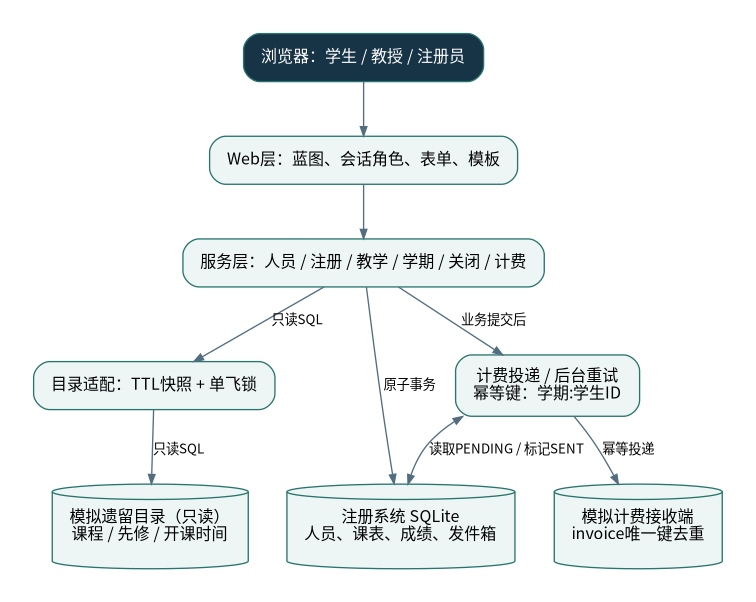
\includegraphics[width=\linewidth,height=.77\textheight,keepaspectratio]{../diagrams/architecture.png}\end{center}\clearpage
\subsection{原始八用例及系统边界}\begin{center}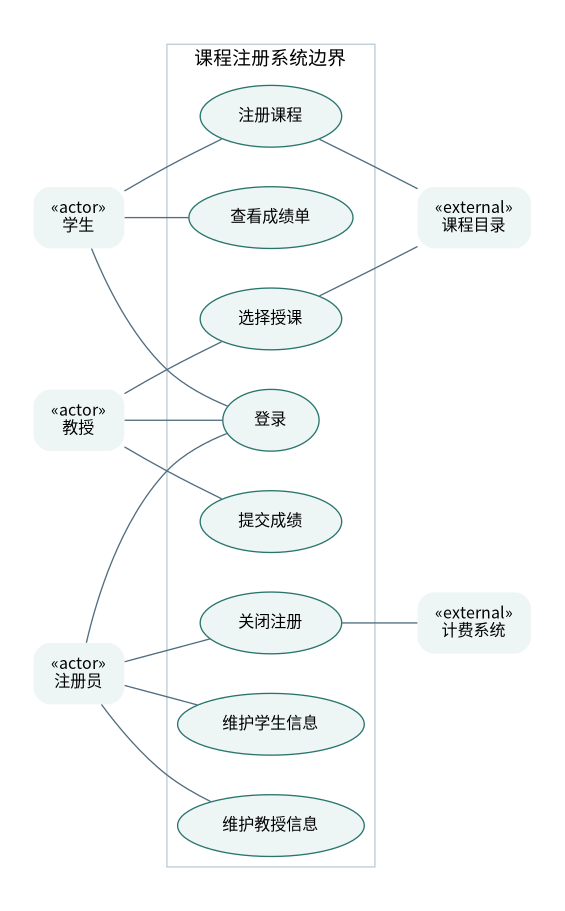
\includegraphics[width=\linewidth,height=.77\textheight,keepaspectratio]{../diagrams/use-cases.png}\end{center}\clearpage
\subsection{领域模型与关联基数}\begin{center}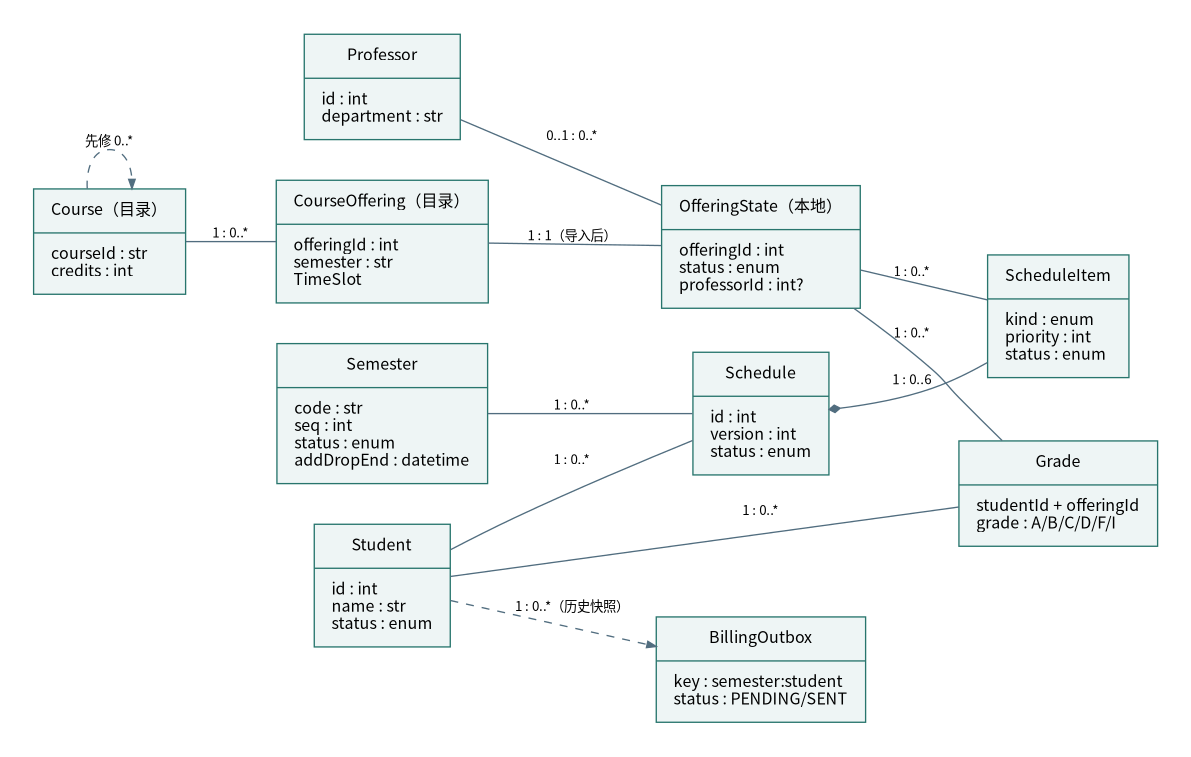
\includegraphics[width=\linewidth,height=.77\textheight,keepaspectratio]{../diagrams/domain-model.png}\end{center}\clearpage
\subsection{学期注册状态机}\begin{center}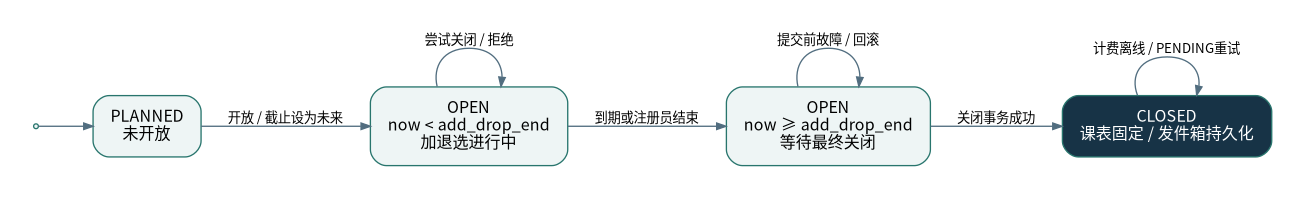
\includegraphics[width=\linewidth,height=.77\textheight,keepaspectratio]{../diagrams/semester-state.png}\end{center}\clearpage
\subsection{提交课表活动流程}\begin{center}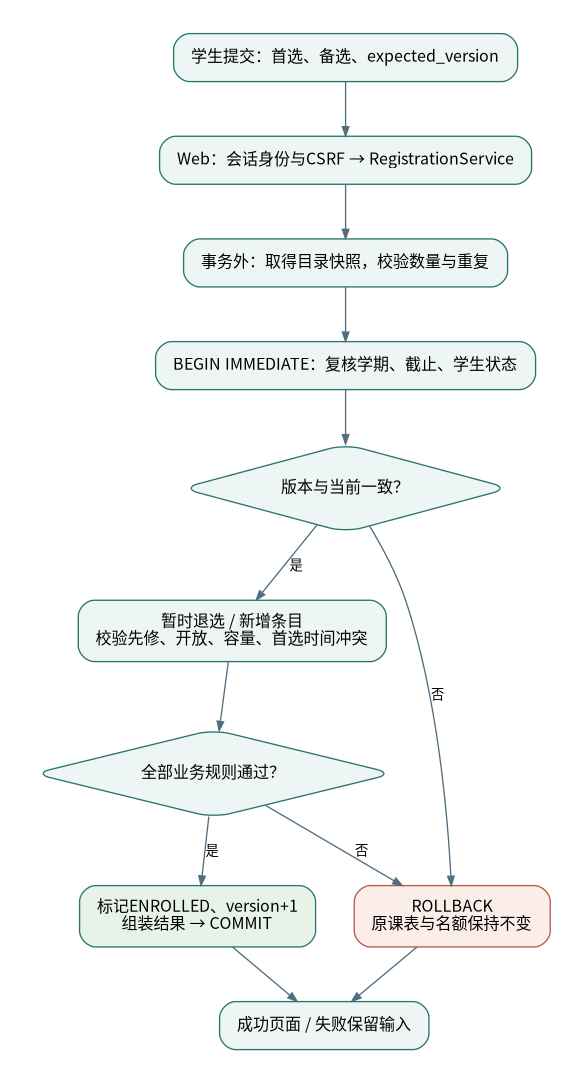
\includegraphics[width=\linewidth,height=.77\textheight,keepaspectratio]{../diagrams/registration-sequence.png}\end{center}\clearpage
\subsection{五人协作依赖}\begin{center}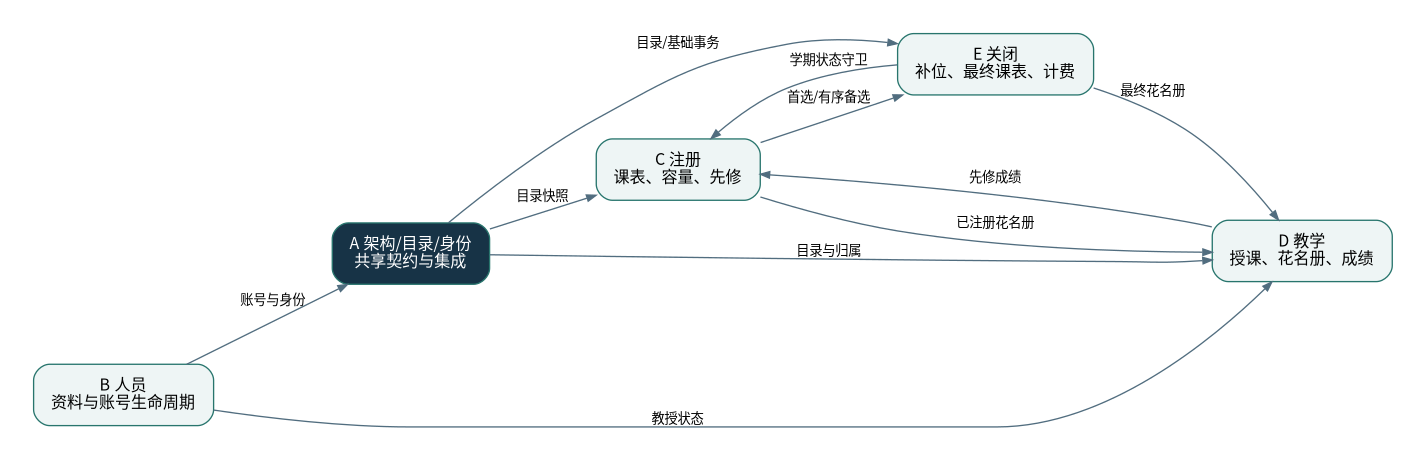
\includegraphics[width=\linewidth,height=.77\textheight,keepaspectratio]{../diagrams/collaboration.png}\end{center}\clearpage
\end{document}